\section{Random variables}

%%%%%%%%%%%%%%%%%%%%%%%%%%%%%%%%%%%%

\begin{frame}
\frametitle{Random variables}

\begin{itemize}

\item A \hl{random variable} is a numeric quantity whose value depends on the outcome of a random event
\begin{itemize}
\item We use a capital letter, like $X$, to denote a random variable
\item The values of a random variable are denoted with a lower case letter, in this case $x$
\item For example, $P(X = x)$
\end{itemize}

\item There are two types of random variables:
\begin{itemize}
\item \hl{Discrete random variables} often take only integer values
\begin{itemize}
\item Example: Number of credit hours, Difference in number of credit hours this term vs last
\end{itemize}
\item \hl{Continuous random variables} take real (decimal) values
\begin{itemize}
\item Example: Cost of books this term, Difference in cost of books this term vs last
\end{itemize}
\end{itemize}

\end{itemize}

\end{frame}

%%%%%%%%%%%%%%%%%%%%%%%%%%%%%%%%%%%%

\subsection{Expectation}

%%%%%%%%%%%%%%%%%%%%%%%%%%%%%%%%%%%%

\begin{frame}
\frametitle{Expectation}

\begin{itemize}

\item We are often interested in the average outcome of a random variable.

\item We call this the \hl{expected value} (mean), and it is a weighted average of the possible outcomes
\formula{\[\mu = E(X) = \sum_{i = 1}^k x ~ P(X = x_i)\]}

\end{itemize}

\end{frame}

%%%%%%%%%%%%%%%%%%%%%%%%%%%%%%%%%%%%

\begin{frame}
\frametitle{Expected value of a discrete random variable}

\dq{In a game of cards you win \$1 if you draw a heart, \$5 if you draw an ace (including the ace of hearts), \$10 if you draw the king of spades and nothing for any other card you draw. Write the probability model for your winnings, and calculate your expected winning.}

\pause

\begin{center}
\renewcommand{\arraystretch}{1.5}
\begin{tabular}{l | c | c | c }
Event		& $X$ 		& $P(X)$        		& $X ~ P(X)$ \\
\hline
Heart (not ace)	& $1$		& $\frac{12}{52}$	& $\frac{12}{52}$ \\
Ace			& $5$		& $\frac{4}{52}$	& $\frac{20}{52}$ \\	
King of spades	& $10$		& $\frac{1}{52}$	& $\frac{10}{52}$ \\	
All else		& $0$		& $\frac{35}{52}$	& $0$ \\
\hline
Total			&			&				& $E(X) = \frac{42}{52} \approx 0.81$
\end{tabular}

\end{center}

\end{frame}

%%%%%%%%%%%%%%%%%%%%%%%%%%%%%%%%%%%%

\begin{frame}
\frametitle{Expected value of a discrete random variable (cont.)}

Below is a visual representation of the probability distribution of winnings from this game:

\begin{center}
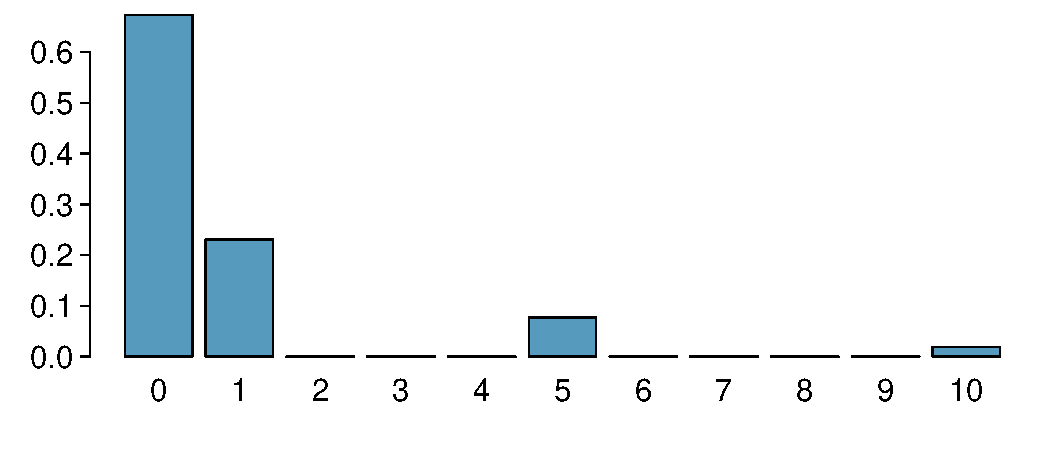
\includegraphics[width=0.8\textwidth]{2-4_random_variables/figures/card_game/card_game}
\end{center}

\end{frame}

%%%%%%%%%%%%%%%%%%%%%%%%%%%%%%%%%%%%

\subsection{Variability in random variables}

%%%%%%%%%%%%%%%%%%%%%%%%%%%%%%%%%%%%

\begin{frame}
\frametitle{Variability}

We are also often interested in the variability in the values of a random variable.

\formula{
\[ \sigma^2 = Var(X) = \sum_{i = 1}^k (x_i - E(X))^2 P(X = x_i) \]
\[ \sigma = SD(X) = \sqrt{Var(X)} \]
}

\end{frame}

%%%%%%%%%%%%%%%%%%%%%%%%%%%%%%%%%%%%

\begin{frame}
\frametitle{Variability of a discrete random variable}

\dq{For the previous card game example, how much would you expect the winnings to vary from game to game?}

\vspace{2mm}
\only<2->{
{\footnotesize
\begin{center}
\renewcommand{\arraystretch}{2}
\begin{tabular}{c | c | c | l | p{4cm}}
$X$ & $P(X)$         & $X ~ P(X)$      & \multicolumn{1}{c|}{$(X - E(X))^2$}  & \multicolumn{1}{c}{$P(X) ~ (X - E(X))^2$}  \\
\hline
1 & $\frac{12}{52}$  & $1 \times \frac{12}{52} = \frac{12}{52}$ & $(1 - 0.81)^2 = 0.0361$ &  $\frac{12}{52} \times 0.0361 = 0.0083$ \\
\hline
5 & $\frac{4}{52}$   & $5 \times \frac{4}{52} = \frac{20}{52}$ & $(5 - 0.81)^2 = 17.5561$  & $\frac{4}{52} \times 17.5561 = 1.3505$ \\
\hline
10  & $\frac{1}{52}$ & $10 \times \frac{1}{52} = \frac{10}{52}$  & $(10 - 0.81)^2 = 84.4561$   & $\frac{1}{52} \times 84.0889 = 1.6242$ \\
\hline
0 & $\frac{35}{52}$  & $0 \times \frac{35}{52} = 0$  & $(0 - 0.81)^2 = 0.6561$ & $\frac{35}{52} \times 0.6561 = 0.4416$ \\
\hline
  &       & $E(X) = 0.81$ & & \soln{\only<3->{$V(X) = 3.4246$}} \\
 &       &                                                         & & \soln{\only<4>{$SD(X) = \sqrt{3.4246} = 1.85$}} \\
\end{tabular}
\end{center}
}
}
\end{frame}

%%%%%%%%%%%%%%%%%%%%%%%%%%%%%%%%%%%%

\subsection{Linear combinations of random variables}

%%%%%%%%%%%%%%%%%%%%%%%%%%%%%%%%%%%%

\begin{frame}
\frametitle{Linear combinations}

\begin{itemize}

\item A \hl{linear combination} of random variables $X$ and $Y$ is given by

\[ aX + bY \]

where $a$ and $b$ are some fixed numbers.

\pause

\item The average value of a linear combination of random variables is given by
\formula{\[ E(aX + bY) = a \times E(X) + b \times E(Y) \]}

\end{itemize}

\end{frame}

%%%%%%%%%%%%%%%%%%%%%%%%%%%%%%%%%%%%

\begin{frame}
\frametitle{Calculating the expectation of a linear combination}

\dq{On average you take 10 minutes for each statistics homework problem and 15 minutes for each chemistry homework problem. This week you have 5 statistics and 4 chemistry homework problems assigned. What is the total time you expect to spend on statistics and physics homework for the week?}

\soln{
\pause
\begin{align*} 
E(5S + 4C) &= 5 \times E(S) + 4 \times E(C) \\
&= 5 \times 10 + 4 \times 15 \\
&= 50 + 60 \\
&= 110~min 
\end{align*}
}

\end{frame}

%%%%%%%%%%%%%%%%%%%%%%%%%%%%%%%%%%%%

\subsection{Variability in linear combinations of random variables}

%%%%%%%%%%%%%%%%%%%%%%%%%%%%%%%%%%%%

\begin{frame}
\frametitle{Linear combinations}

\begin{itemize}

\item The variability of a linear combination of two independent random variables is calculated as
\formula{\[ V(aX + bY) = a^2 \times V(X) + b^2 \times V(Y) \]}

\pause 

\item The standard deviation of the linear combination is the square root of the variance.

\end{itemize}

\pause 
\vfill

\Note{If the random variables are not independent, the variance calculation gets a little more complicated and is beyond the scope of this course.}

\end{frame}

%%%%%%%%%%%%%%%%%%%%%%%%%%%%%%%%%%%%

\begin{frame}
\frametitle{Calculating the variance of a linear combination}

\dq{The standard deviation of the time you take for each statistics homework problem is 1.5 minutes, and it is 2 minutes for each chemistry problem. What is the standard deviation of the time you expect to spend on statistics and physics homework for the week if you have 5 statistics and 4 chemistry homework problems assigned?}

\soln{
\pause
\begin{align*} 
V(5S + 4C) &= 5^2 \times V(S) + 4^2 \times V(C) \\
&= 25 \times 1.5^2 + 16 \times 2^2 \\
&= 56.25 + 64 \\
&= 120.25 
\end{align*}
}

\end{frame}

%%%%%%%%%%%%%%%%%%%%%%%%%%%%%%%%%%%%

\subsection{Recap}

%%%%%%%%%%%%%%%%%%%%%%%%%%%%%%%%%%%%

\begin{frame}
\frametitle{Practice}

\pq{A casino game costs \$5 to play. If you draw first a red card, then you get to draw a second card. If the second card is the ace of hearts, you win \$500. If not, you don't win anything, i.e. lose your \$5. What is your expected profits/losses from playing this game? {\small Remember: profit/loss = winnings - cost.}}

\begin{multicols}{2}
\begin{enumerate}[(a)]
\item A loss of 10\textcent
\item A loss of 25\textcent
\solnMult{A loss of 30\textcent}
\item A profit of 5\textcent
\end{enumerate}
\end{multicols}

\soln{
\only<2>{
{\small
\renewcommand\arraystretch{1.25}
\begin{tabular}{l c c c r}
Event				& Win	& Profit: $X$	& $P(X)$	& $ X \times P(X)$	\\
\hline
\red{Red}, \red{A}\red{$\varheartsuit$}		& 500		& 500 - 5 = 495	& $\frac{25}{52} \times \frac{1}{51} = 	0.0094$ & 	 $495 \times 0.0094 = 4.653$ \\
Other	& 0 			& 0 - 5 = -5	& $1 - 0.0094 = 0.9906$ & $-5 \times 0.9906 = -4.953$ \\  
\hline
					&			&			& 			& $E(X) = -0.3$
\end{tabular}
}
}
}

\end{frame}

%%%%%%%%%%%%%%%%%%%%%%%%%%%%%%%%%%%%

\begin{frame}
\frametitle{Fair game}

A \hl{fair} game is defined as a game that costs as much as its expected payout, i.e. expected profit is 0.

\pause

$\:$

\dq{Do you think casino games in Vegas cost more or less than their expected payouts?}

\soln{
\pause
\begin{columns}[c]
\column{0.6\textwidth}
If those games cost less than their expected payouts, it would mean that the casinos would be losing money on average, and hence they wouldn't be able to pay for all this:
\column{0.4\textwidth}
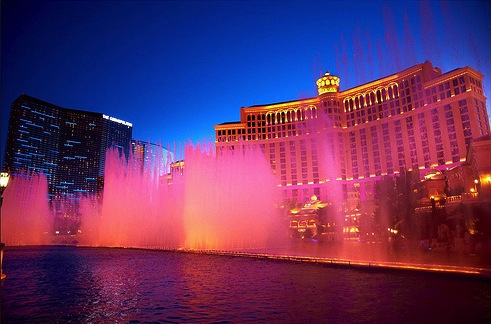
\includegraphics[width=\textwidth]{2-4_random_variables/figures/bellagio.jpg}
\end{columns}
\ct{Image by Moyan\_Brenn on Flickr \webURL{http://www.flickr.com/photos/aigle\_dore/5951714693}.}
}


\end{frame}

%%%%%%%%%%%%%%%%%%%%%%%%%%%%%%%%%%%%%

\begin{frame}
\frametitle{Simplifying random variables}

Random variables do not work like normal algebraic variables:
\[ X + X \ne 2X \]

\pause

{\small
\twocol{0.45}{0.45}
{
\begin{align*}
E(X + X) &= E(X) + E(X) \\
&= 2 E(X) \\
&~  \\
E(2X) &= 2 E(X) \\
&~ 
\end{align*}
}
{
\begin{align*}
Var(X + X) &= Var(X) + Var(X)~{\scriptsize \text{(assuming independence)}} \\
&= 2~Var(X) \\
&~  \\
Var(2X) &= 2^2~Var(X) \\
&= 4~Var(X)
\end{align*}
}
}


\pause

\vspace{3mm}

\mathhl{E(X + X)  = E(2X)}, but \mathhl{Var(X + X) \ne Var(2X)}.

\end{frame}

%%%%%%%%%%%%%%%%%%%%%%%%%%%%%%%%%%%%%

\begin{frame}
\frametitle{Adding or multiplying?}

\dq{A company has 5 Lincoln Town Cars in its fleet. Historical data show that annual maintenance cost for each car is on average \$2,154 with a standard deviation of \$132. What is the mean and the standard deviation of the total annual maintenance cost for this fleet?}

\pause

Note that we have 5 cars each with the given annual maintenance cost $(X_1 + X_2 + X_3 + X_4 + X_5)$, not one car that had 5 times the given annual maintenance cost $(5X)$.

\pause

{\small
\begin{eqnarray*} 
E(X_1 + X_2 + X_3 + X_4 + X_5) &=& E(X_1) + E(X_2) + E(X_3) + E(X_4) + E(X_5) \\
\pause
&=& 5 \times E(X) = 5 \times 2,154 = \$ 10,770 \\
\pause
Var(X_1 + X_2 + X_3 + X_4 + X_5) &=& Var(X_1) + Var(X_2) + Var(X_3) + Var(X_4) + Var(X_5) \\
\pause
&=& 5 \times V(X) = 5 \times 132^2 = \$ 87,120 \\
\pause
SD(X_1 + X_2 + X_3 + X_4 + X_5) &=& \sqrt{87,120} =  295.16
\end{eqnarray*}
}

\end{frame}

